\documentclass[article]{jss}

\RequirePackage{color,fancyvrb,amsmath,amsfonts}
\usepackage{doBy-JSS}

%%%%%%%%%%%%%%%%%%%%%%%%%%%%%%
%% declarations for jss.cls %%%%%%%%%%%%%%%%%%%%%%%%%%%%%%%%%%%%%%%%%%
%%%%%%%%%%%%%%%%%%%%%%%%%%%%%%

%% almost as usual
\author{Ulrich Halekoh\\ Aarhus University \And 
        S�ren H�jsgaard \\ Aalborg University}
\title{
  Tools for Applied Statistics -- the \doby\ Package
}

  
%% for pretty printing and a nice hypersummary also set:
\Plainauthor{Ulrich Halekoh, S�ren H�jsgaard} %% comma-separated
\Plaintitle{The doBy package} %% without formatting
%%\Shorttitle{Test in mixed models} %% a short title (if necessary)

%% an abstract and keywords
\Abstract{
}
\Keywords{}

\Plainkeywords{keywords, comma-separated, not capitalized, Java} %% without formatting
%% at least one keyword must be supplied

%% publication information
%% NOTE: Typically, this can be left commented and will be filled out by the technical editor
%% \Volume{13}
%% \Issue{9}
%% \Month{September}
%% \Year{2004}
%% \Submitdate{2004-09-29}
%% \Acceptdate{2004-09-29}

%% The address of (at least) one author should be given
%% in the following format:



\Address{
  Ulrich Halekoh\\
  Department of Animal Health and Bioscience\\
  Aarhus University\\
  Blichers All�, 8830 Tjele, Denmark\\
  E-mail: \email{ulrich.halekoh@agrsci.dk}
\\
  S�ren H�jsgaard\\
  Department of Mathematical Sciences\\
  Aalborg University\\
  Fredrik Bajers Vej 7G, 9220 Aalborg �, Denmark\\
  E-mail: \email{sorenh@math.aau.dk}\\
  URL: \url{http://people.math.aau.dk/~sorenh/}

}

%% It is also possible to add a telephone and fax number
%% before the e-mail in the following format:
%% Telephone: +43/1/31336-5053
%% Fax: +43/1/31336-734

%% for those who use Sweave please include the following line (with % symbols):
%% need no \usepackage{Sweave.sty}

%% end of declarations %%%%%%%%%%%%%%%%%%%%%%%%%%%%%%%%%%%%%%%%%%%%%%%


\usepackage{color}
\usepackage[inline,nomargin,draft]{fixme}
% \newcommand\FXInline[2]{\textbf{\color{blue}#1}:
%   \emph{\color{blue} - #2}}


\begin{document}

%\renewenvironment{Schunk}{\linespread{.85}\small}{}
 
\setkeys{Gin}{width=0.5\textwidth} %s�t figurst�rrelse i Sweave

%\fxnote{where should this line be placesd?}





\section{Introduction}
\label{sec:intro}



\def\doby{\pkg{doBy}}
\def\code#1{\texttt{#1}}
\def\summaryby{\code{summaryBy()}}
\def\R{\proglang{R}}


%\parindent0pt\parskip5pt

\section{Introduction}
\label{sec:introduction}

The \doby\ package, \citep{doBy} for \R, \citep{R} contains a variety
of utility functions. The package grew out of many years of work in
biostatistics; in particular in agricultural sciences. This paper
describes some of the functions in \doby. \fxnote{May want to mention
  a few other utility packages on CRAN.}




\section{Data used for illustration}
\label{sec:co2data}

The description of the \code{doBy} package is based on the following
datasets.

\paragraph{CO2 data}

The \code{CO2} data frame comes  from an
experiment on the cold tolerance of the grass species {\em Echinochloa
crus-galli}.
To limit the amount of output we modify names and levels of variables
as follows

\begin{Schunk}
\begin{Sinput}
R> data(CO2)
R> CO2 <- transform(CO2, Treat=Treatment, Treatment=NULL)
R> levels(CO2$Treat) <- c("nchil","chil")
R> levels(CO2$Type)  <- c("Que","Mis")
R> CO2 <- subset(CO2, Plant %in% c("Qn1", "Qc1", "Mn1", "Mc1"))
R> head(CO2)
\end{Sinput}
\begin{Soutput}
  Plant Type conc uptake Treat
1   Qn1  Que   95   16.0 nchil
2   Qn1  Que  175   30.4 nchil
3   Qn1  Que  250   34.8 nchil
4   Qn1  Que  350   37.2 nchil
5   Qn1  Que  500   35.3 nchil
6   Qn1  Que  675   39.2 nchil
\end{Soutput}
\end{Schunk}

% Data is shown in Section~\ref{sec:appdata}.


\paragraph{Airquality data}

The \code{airquality}
dataset contains  air quality measurements in New York, May to
September 1973. The months are coded as $5,\dots,9$.
To limit the output we only consider data for two months:
\begin{Schunk}
\begin{Sinput}
R> airquality <- subset(airquality, Month %in% c(5,6))
R> head(airquality)
\end{Sinput}
\begin{Soutput}
  Ozone Solar.R Wind Temp Month Day
1    41     190  7.4   67     5   1
2    36     118  8.0   72     5   2
3    12     149 12.6   74     5   3
4    18     313 11.5   62     5   4
5    NA      NA 14.3   56     5   5
6    28      NA 14.9   66     5   6
\end{Soutput}
\end{Schunk}
%Data is shown in Section~\ref{sec:appdata}.

% \paragraph{Dietox data}
% The \code{dietox} data are provided in the \code{doBy} package and
% result from a study of the effect of adding vitamin E and/or copper to
% the feed of slaughter pigs.


\section{Working with groupwise data}

\subsection[]{Univariate summary statistics -- The \summaryby\ function}
\label{sec:summaryBy}

The \summaryby{} function is used for calculating quantities like
``the mean and variance of $x$ and $y$ for
each combination of two factors $A$ and $B$''. Examples are based on
the \code{CO2} data.


\subsubsection{Basic usage}
\label{sec:xxx}


For example, the mean and variance of \code{uptake} and
\code{conc} for each value of \code{Plant} is obtained by:
\begin{Schunk}
\begin{Sinput}
R> myfun1 <- function(x){c(m=mean(x), s=sd(x), sem=sd(x)/length(x))}
R> summaryBy(conc + uptake ~ Plant, data=CO2, FUN=myfun1)
\end{Sinput}
\begin{Soutput}
  Plant conc.m conc.s conc.sem uptake.m uptake.s uptake.sem
1   Qn1    435  317.7    45.39    33.23    8.215     1.1735
2   Qc1    435  317.7    45.39    29.97    8.335     1.1907
3   Mn1    435  317.7    45.39    26.40    8.694     1.2420
4   Mc1    435  317.7    45.39    18.00    4.119     0.5884
\end{Soutput}
\end{Schunk}

Defining the function to return named values as above is the
recommended use of \summaryby.
Note that the values returned by the function has been named as
\code{m} and \code{s}.

If the result of the function(s) are not named, then the names in the
output data in general become less intuitive:
\begin{Schunk}
\begin{Sinput}
R> myfun2 <- function(x){c(mean(x), var(x), sd(x)/length(x))}
R> summaryBy(conc + uptake ~ Plant, data=CO2, FUN=myfun2)
\end{Sinput}
\begin{Soutput}
  Plant conc.FUN1 conc.FUN2 conc.FUN3 uptake.FUN1 uptake.FUN2
1   Qn1       435    100950     45.39       33.23       67.48
2   Qc1       435    100950     45.39       29.97       69.47
3   Mn1       435    100950     45.39       26.40       75.59
4   Mc1       435    100950     45.39       18.00       16.96
  uptake.FUN3
1      1.1735
2      1.1907
3      1.2420
4      0.5884
\end{Soutput}
\end{Schunk}



\subsubsection{Using predefined functions}
\label{sec:xxx}


It is possible use a vector of predefined functions. For example
\begin{Schunk}
\begin{Sinput}
R> sem <- function(x){sd(x)/length(x)}
R> summaryBy(uptake~Plant, data=CO2, FUN=list(mean,sd,sem,N=length))
\end{Sinput}
\begin{Soutput}
  Plant uptake.mean uptake.sd uptake.sem uptake.length
1   Qn1       33.23     8.215     1.1735             7
2   Qc1       29.97     8.335     1.1907             7
3   Mn1       26.40     8.694     1.2420             7
4   Mc1       18.00     4.119     0.5884             7
\end{Soutput}
\end{Schunk}

The naming of the output variables determined from what the functions
returns. The names of the last two columns above are imposed
by \summaryby{} because \code{myfun2} does not return named values.



% \subsubsection[]{Naming output variables with the \code{postfix} argument}
% \label{sec:postfix}

% The \code{postfix} argument gives an altertive way of naming the
% output variables: For example, the functions \code{myfun1} and
% \code{myfun2} both returns
% two values. These can be named as:
% @
% <<>>=
% summaryBy(conc+uptake~Plant, data=CO2, postfix=list(
% c("mean1", "var1"),c("mean2", "var2")),
% FUN=c(myfun1,myfun2))
% @ %def

% Specifying \code{postfix=} overrides these names but when \code{FUN}
% is a list of functions, the new names are not very informative
% either:\footnote{This may be improved on later.}
% @
% <<>>=
% summaryBy(uptake~Plant, data=CO2,
% postfix=c("aa","bb","cc"),
% FUN=c(mean,var,myfun1,myfun2))
% @ %def

\subsubsection[]{Copying variables out with the \code{id} argument}
\label{sec:xxx}

To get the value of the \code{Type} and \code{Treat} in the first row of the
groups (defined by the values of \code{Plant}) copied to the output
dataframe we use the \code{id} argument:
as:
\begin{Schunk}
\begin{Sinput}
R> summaryBy(conc+uptake~Plant, data=CO2, FUN=myfun1, id=~Type+Treat)
\end{Sinput}
\begin{Soutput}
  Plant conc.m conc.s conc.sem uptake.m uptake.s uptake.sem Type
1   Qn1    435  317.7    45.39    33.23    8.215     1.1735  Que
2   Qc1    435  317.7    45.39    29.97    8.335     1.1907  Que
3   Mn1    435  317.7    45.39    26.40    8.694     1.2420  Mis
4   Mc1    435  317.7    45.39    18.00    4.119     0.5884  Mis
  Treat
1 nchil
2  chil
3 nchil
4  chil
\end{Soutput}
\end{Schunk}


\subsubsection{Statistics on functions of data}
\label{sec:xxx}
We may want to calculate the mean and variance for the logarithm of
\code{uptake}, for \code{uptake}/\code{conc} and for \code{uptake} and
\code{conc}. This can be achieved as:
\begin{Schunk}
\begin{Sinput}
R> summaryBy(log(uptake)+I(conc/uptake)+ conc+uptake~Plant, data=CO2,
+  FUN=myfun1)
\end{Sinput}
\begin{Soutput}
  Plant log(uptake).m log(uptake).s log(uptake).sem conc/uptake.m
1   Qn1         3.467        0.3189         0.04555         12.12
2   Qc1         3.356        0.3446         0.04922         13.23
3   Mn1         3.209        0.4234         0.06049         14.92
4   Mc1         2.864        0.2622         0.03746         22.12
  conc/uptake.s conc/uptake.sem conc.m conc.s conc.sem uptake.m
1         7.204           1.029    435  317.7    45.39    33.23
2         7.195           1.028    435  317.7    45.39    29.97
3         7.312           1.045    435  317.7    45.39    26.40
4        12.883           1.840    435  317.7    45.39    18.00
  uptake.s uptake.sem
1    8.215     1.1735
2    8.335     1.1907
3    8.694     1.2420
4    4.119     0.5884
\end{Soutput}
\end{Schunk}

If one does not want output variables to contain parentheses then
setting \code{p2d=TRUE} causes the parentheses to be replaced by dots
(``.'').
% @
% <<>>=
% summaryBy(log(uptake)+I(conc+uptake)~Plant, data=CO2, p2d=TRUE,
% FUN=myfun1)
% @ %def






\subsubsection{Using '.' ans '1' in the specifications}
\label{sec:xxx}

It is possible  to use the dot (".") on the left hand side of
the formula. The dot means "all numerical variables which do not
appear elsewhere" (i.e.\ on the right hand side of the formula and in
the \code{id} statement):
\begin{Schunk}
\begin{Sinput}
R> summaryBy(log(uptake) + I(conc/uptake) + . ~Plant, data=CO2, FUN=myfun1)
\end{Sinput}
\begin{Soutput}
  Plant log(uptake).m log(uptake).s log(uptake).sem conc/uptake.m
1   Qn1         3.467        0.3189         0.04555         12.12
2   Qc1         3.356        0.3446         0.04922         13.23
3   Mn1         3.209        0.4234         0.06049         14.92
4   Mc1         2.864        0.2622         0.03746         22.12
  conc/uptake.s conc/uptake.sem conc.m conc.s conc.sem uptake.m
1         7.204           1.029    435  317.7    45.39    33.23
2         7.195           1.028    435  317.7    45.39    29.97
3         7.312           1.045    435  317.7    45.39    26.40
4        12.883           1.840    435  317.7    45.39    18.00
  uptake.s uptake.sem
1    8.215     1.1735
2    8.335     1.1907
3    8.694     1.2420
4    4.119     0.5884
\end{Soutput}
\end{Schunk}

The dot (".") can also be used on the right hand side of the formula
where it refers to "all non--numerical variables which are not
specified elsewhere":
\begin{Schunk}
\begin{Sinput}
R> summaryBy(log(uptake) ~ Plant + ., data=CO2, FUN=myfun1)
\end{Sinput}
\begin{Soutput}
  Plant Type Treat log(uptake).m log(uptake).s log(uptake).sem
1   Qn1  Que nchil         3.467        0.3189         0.04555
2   Qc1  Que  chil         3.356        0.3446         0.04922
3   Mn1  Mis nchil         3.209        0.4234         0.06049
4   Mc1  Mis  chil         2.864        0.2622         0.03746
\end{Soutput}
\end{Schunk}


Using 1 on the
  right hand side means no grouping:
\begin{Schunk}
\begin{Sinput}
R> summaryBy(log(uptake) ~ 1, data=CO2, FUN=myfun1)
\end{Sinput}
\begin{Soutput}
  log(uptake).m log(uptake).s log(uptake).sem
1         3.224        0.3971         0.01418
\end{Soutput}
\end{Schunk}

\fxnote{Should be possible to supply first argument as a list}


\subsubsection[]{Preserving names of variables using \code{keep.names}}
\label{sec:xxx}
If the function applied to data only returns one value, it is possible
to force that the summary variables retain the original names by
setting \code{keep.names=TRUE}. A
typical use of this could be
\begin{Schunk}
\begin{Sinput}
R> summaryBy(conc+uptake+log(uptake)~Plant,
+  data=CO2, FUN=mean, id=~Type+Treat, keep.names=TRUE)
\end{Sinput}
\begin{Soutput}
  Plant conc uptake log(uptake) Type Treat
1   Qn1  435  33.23       3.467  Que nchil
2   Qc1  435  29.97       3.356  Que  chil
3   Mn1  435  26.40       3.209  Mis nchil
4   Mc1  435  18.00       2.864  Mis  chil
\end{Soutput}
\end{Schunk}


\def\orderby{\code{orderBy()}}
\subsection[]{The \orderby\ function}
\label{orderBy}

Ordering (or sorting) a data frame is possible with the \orderby\ 
function.
Suppose we want to order the rows of the the \code{airquality} data by
\code{Temp} (in decreasing order) and by
\code{Month} (within \code{Temp}). This can be achieved by:
\begin{Schunk}
\begin{Sinput}
R> x <- orderBy(~ -Temp + Month, data=airquality)
R> head(x)
\end{Sinput}
\begin{Soutput}
   Ozone Solar.R Wind Temp Month Day
42    NA     259 10.9   93     6  11
43    NA     250  9.2   92     6  12
40    71     291 13.8   90     6   9
39    NA     273  6.9   87     6   8
41    39     323 11.5   87     6  10
36    NA     220  8.6   85     6   5
\end{Soutput}
\end{Schunk}



\subsection[]{The \code{splitBy()} function}
\label{splitBy}

Suppose we want to split the \code{airquality} data into a list of
dataframes with one
dataframe for every half month. This can be achieved by:
\begin{Schunk}
\begin{Sinput}
R> airquality <- transform(airquality, wim=Day>15)
R> ss<-splitBy(~Month + wim, data=airquality)
R> ss
\end{Sinput}
\begin{Soutput}
  listentry Month   wim
1   5|FALSE     5 FALSE
2    5|TRUE     5  TRUE
3   6|FALSE     6 FALSE
4    6|TRUE     6  TRUE
\end{Soutput}
\end{Schunk}
Hence for month 5, the relevant entry-name in the list is '5' and this
part of data  can
be extracted as
\begin{Schunk}
\begin{Sinput}
R> ss[['5|FALSE']]
\end{Sinput}
\end{Schunk}


Information about the grouping is stored as a dataframe
in an attribute called \code{groupid} and can be retrieved with:
\begin{Schunk}
\begin{Sinput}
R> attr(ss,"groupid")
\end{Sinput}
\begin{Soutput}
  Month   wim
1     5 FALSE
2     5  TRUE
3     6 FALSE
4     6  TRUE
\end{Soutput}
\end{Schunk}

\fxnote{listentry er dumt navn. forklar ogs� at resultatet er en liste...}

\subsection[]{The \code{subsetBy()} function}
\label{subsetBy}

Suppose we want to select those rows within each month for which the the
wind speed is larger than the mean wind speed (within the month). This
is achieved by:
\begin{Schunk}
\begin{Sinput}
R> subsetBy(~Month, subset=Wind > mean(Wind), data=airquality)
\end{Sinput}
\end{Schunk}
Note that the statement \code{Wind > mean(Wind)} is evaluated within
each month.



\subsection[]{The \code{transformBy} function}
\label{sec:transformby}

The \code{transformBy} function is analogous to the \code{transform}
function except that it works within groups. For example:
\begin{Schunk}
\begin{Sinput}
R> zz<- transformBy(~Month, data=airquality, minW=min(Wind), maxW=max(Wind),
+       chg=sum(range(Wind)*c(-1,1)))
R> head(zz)
\end{Sinput}
\begin{Soutput}
    Ozone Solar.R Wind Temp Month Day   wim minW maxW  chg
5.1    41     190  7.4   67     5   1 FALSE  5.7 20.1 14.4
5.2    36     118  8.0   72     5   2 FALSE  5.7 20.1 14.4
5.3    12     149 12.6   74     5   3 FALSE  5.7 20.1 14.4
5.4    18     313 11.5   62     5   4 FALSE  5.7 20.1 14.4
5.5    NA      NA 14.3   56     5   5 FALSE  5.7 20.1 14.4
5.6    28      NA 14.9   66     5   6 FALSE  5.7 20.1 14.4
\end{Soutput}
\end{Schunk}


\def\lapplyby{\texttt{lapplyBy()}}

\subsection[]{The \lapplyby\ function}
\label{sec:transformby}

The \lapplyby\ function is a wrapper for first splitting data
into a list according to the formula (using \code{splitBy()}) and then applying
a function to each element of the list (using \code{apply()}).
Consider the \code{CO2} data. Suppose that for each plant we want to
find the change in \code{uptake} per change in \code{conc}:

\begin{Schunk}
\begin{Sinput}
R> CO2 <- orderBy(~Plant + conc, data=CO2)
R> vv <- lapplyBy(~ Plant, data=CO2, 
+                 FUN = function(x){c(NA, diff(x$uptake) / diff(x$conc))})
R> str(vv)
\end{Sinput}
\begin{Soutput}
List of 4
 $ Qn1: num [1:7] NA 0.18 0.0587 0.024 -0.0127 ...
 $ Qc1: num [1:7] NA 0.1238 0.0827 0.043 -0.014 ...
 $ Mn1: num [1:7] NA 0.1075 0.0933 0.038 0.006 ...
 $ Mc1: num [1:7] NA 0.055 0.0427 0.008 0.004 ...
\end{Soutput}
\end{Schunk}




\subsection[]{The \code{sampleBy()} function}
\label{sampleBy}

Suppose we want a random sample of 50 \% of the observations from a
dataframe. This can be achieved with:
\begin{Schunk}
\begin{Sinput}
R> sampleBy(~1, frac=0.5, data=airquality)
\end{Sinput}
\end{Schunk}

Suppose instead that we want a  systematic sample of  every fifth
observation within each month. This is achieved with:
\begin{Schunk}
\begin{Sinput}
R> sampleBy(~Month, frac=0.2, data=airquality,systematic=T)
\end{Sinput}
\end{Schunk}




% \subsection{Example: using \code{splitBy()}}
% \label{sec:exampl-using-codespl}

% @
% <<>>=
% CO2.lst <- splitBy(~Type+Treat, data=CO2)
% CO2.lst
% @ %def

% @
% <<>>=
% wd <- CO2.lst[[1]] ## wd : "working data"
% wd$l.fit <- fitted(with(wd, loess(uptake~conc)))
% @ %def

% @
% <<>>=
% CO2.lst2 <- lapplyBy(~Type+Treat, data=CO2, FUN=function(wd){
%     wd$l.fit <- fitted(with(wd, loess(uptake~conc)))
%     wd
% })
% @


% <<fig=T>>=
% par(mfrow=c(2,2))
% lapply(CO2.lst2, function(wd){
%     plot(uptake~conc, data=wd)
%     lines(l.fit~conc, data=wd)
% })
% @ %def










\section{Miscellaneous}
\label{sec:xxx}


\subsection[]{The \code{firstobs()} / \code{lastobs()} function}
\label{firstlast}

To obtain the indices of the first/last occurences of an item in a
vector do:
\begin{Schunk}
\begin{Sinput}
R> x <- c(1,1,1,2,2,2,1,1,1,3)
R> firstobs(x)
\end{Sinput}
\begin{Soutput}
[1]  1  4 10
\end{Soutput}
\begin{Sinput}
R> lastobs(x)
\end{Sinput}
\begin{Soutput}
[1]  6  9 10
\end{Soutput}
\end{Schunk}

The same can be done on a data frame, e.g.
\begin{Schunk}
\begin{Sinput}
R> firstobs(~Plant, data=CO2)
\end{Sinput}
\begin{Soutput}
[1]  1  8 15 22
\end{Soutput}
\begin{Sinput}
R> lastobs(~Plant, data=CO2)
\end{Sinput}
\begin{Soutput}
[1]  7 14 21 28
\end{Soutput}
\end{Schunk}

\subsection[]{The \code{which.maxn()} and \code{which.minn()} functions}
\label{sec:whichmaxn}

The location of the $n$ largest / smallest entries in a numeric vector
can be obtained with
\begin{Schunk}
\begin{Sinput}
R> x <- c(1:4,0:5,11,NA,NA)
R> which.maxn(x,3)
\end{Sinput}
\begin{Soutput}
[1] 11 10  4
\end{Soutput}
\begin{Sinput}
R> which.minn(x,5)
\end{Sinput}
\begin{Soutput}
[1] 5 1 6 2 7
\end{Soutput}
\end{Schunk}

\subsection[]{Subsequences - \code{subSeq()}}
\label{sec:xxx}

Find (sub) sequences in a vector:

\begin{Schunk}
\begin{Sinput}
R> x <- c(1,1,2,2,2,1,1,3,3,3,3,1,1,1)
R> subSeq(x)
\end{Sinput}
\begin{Soutput}
  first last slength midpoint value
1     1    2       2        2     1
2     3    5       3        4     2
3     6    7       2        7     1
4     8   11       4       10     3
5    12   14       3       13     1
\end{Soutput}
\begin{Sinput}
R> subSeq(x, item=1)
\end{Sinput}
\begin{Soutput}
  first last slength midpoint value
1     1    2       2        2     1
2     6    7       2        7     1
3    12   14       3       13     1
\end{Soutput}
\begin{Sinput}
R> subSeq(letters[x])
\end{Sinput}
\begin{Soutput}
  first last slength midpoint value
1     1    2       2        2     a
2     3    5       3        4     b
3     6    7       2        7     a
4     8   11       4       10     c
5    12   14       3       13     a
\end{Soutput}
\begin{Sinput}
R> subSeq(letters[x],item="a")
\end{Sinput}
\begin{Soutput}
  first last slength midpoint value
1     1    2       2        2     a
2     6    7       2        7     a
3    12   14       3       13     a
\end{Soutput}
\end{Schunk}


\subsection[]{Recoding values of a vector - \code{recodeVar()}}
\label{sec:xxx}

\begin{Schunk}
\begin{Sinput}
R> x <- c("dec","jan","feb","mar","apr","may")
R> src1 <- list(c("dec","jan","feb"), c("mar","apr","may"))
R> tgt1 <- list("winter","spring")
R> recodeVar(x,src=src1,tgt=tgt1)
\end{Sinput}
\begin{Soutput}
[1] "winter" "winter" "winter" "spring" "spring" "spring"
\end{Soutput}
\end{Schunk}

\subsection[]{Renaming columns of a dataframe or matrix --  \code{renameCol()}}
\label{sec:xxx}

\begin{Schunk}
\begin{Sinput}
R> head(renameCol(CO2, 1:2, c("kk","ll")))
\end{Sinput}
\begin{Soutput}
   kk  ll conc uptake Treat
1 Qn1 Que   95   16.0 nchil
2 Qn1 Que  175   30.4 nchil
3 Qn1 Que  250   34.8 nchil
4 Qn1 Que  350   37.2 nchil
5 Qn1 Que  500   35.3 nchil
6 Qn1 Que  675   39.2 nchil
\end{Soutput}
\begin{Sinput}
R> head(renameCol(CO2, c("Plant","Type"), c("kk","ll")))
\end{Sinput}
\begin{Soutput}
   kk  ll conc uptake Treat
1 Qn1 Que   95   16.0 nchil
2 Qn1 Que  175   30.4 nchil
3 Qn1 Que  250   34.8 nchil
4 Qn1 Que  350   37.2 nchil
5 Qn1 Que  500   35.3 nchil
6 Qn1 Que  675   39.2 nchil
\end{Soutput}
\end{Schunk}

\subsection[]{Time since an event - \code{timeSinceEvent()}}
\label{sec:xxx}

Consider the vectors
\begin{Schunk}
\begin{Sinput}
R> yvar <- c(0,0,1,0,0,0,0,0,1,0,0,0,1,1,0,0,0)
R> (tvar <- seq_along(yvar) + c(0.1,0.2))
\end{Sinput}
\begin{Soutput}
 [1]  1.1  2.2  3.1  4.2  5.1  6.2  7.1  8.2  9.1 10.2 11.1 12.2 13.1
[14] 14.2 15.1 16.2 17.1
\end{Soutput}
\end{Schunk}

Imagine that a non--zero element in \code{yvar} indicates an event  which takes place
at the corresponding time point in \code{tvar} (which by default is
assumed to contain equidistant values)

Now we find time since event as
\begin{Schunk}
\begin{Sinput}
R> tse<- timeSinceEvent(yvar,tvar)
\end{Sinput}
\begin{Soutput}
   yvar tvar abs.tse sign.tse ewin run tae  tbe
1     0  1.1     2.0     -2.0    1  NA  NA -2.0
2     0  2.2     0.9     -0.9    1  NA  NA -0.9
3     1  3.1     0.0      0.0    1   1 0.0  0.0
4     0  4.2     1.1      1.1    1   1 1.1 -4.9
5     0  5.1     2.0      2.0    1   1 2.0 -4.0
6     0  6.2     2.9     -2.9    2   1 3.1 -2.9
7     0  7.1     2.0     -2.0    2   1 4.0 -2.0
8     0  8.2     0.9     -0.9    2   1 5.1 -0.9
9     1  9.1     0.0      0.0    2   2 0.0  0.0
10    0 10.2     1.1      1.1    2   2 1.1 -2.9
11    0 11.1     2.0      2.0    2   2 2.0 -2.0
12    0 12.2     0.9     -0.9    3   2 3.1 -0.9
13    1 13.1     0.0      0.0    3   3 0.0  0.0
14    1 14.2     0.0      0.0    4   4 0.0  0.0
15    0 15.1     0.9      0.9    4   4 0.9   NA
16    0 16.2     2.0      2.0    4   4 2.0   NA
17    0 17.1     2.9      2.9    4   4 2.9   NA
\end{Soutput}
\end{Schunk}

The output reads as follows:
\begin{itemize}
\item \verb'abs.tse' and \verb'sign.tse': Absolute and signed time since (nearest) event.
\item \verb'ewin': Event window: Gives a symmetric window around each
  event. \fxnote{ewin beregnes forkert}
\item \verb'run': The value of \verb'run' is set to $1$ when the first
  event occurs and is increased by $1$ at each subsequent event.
\item \verb'tae' and \verb'tbe': Time after and before event.
\end{itemize}


% <<fig=T>>=
% plot(sign.tse~tvar, data=tse, type="b")
% grid()
% rug(tse$tvar[tse$yvar==1], col='blue',lwd=4)
% points(scale(tse$run), col=tse$run, lwd=2)
% lines(abs.tse+.2~tvar, data=tse, type="b",col=3)
% @ %def

% @
% <<fig=T>>=
% plot(tae~tvar, data=tse, ylim=c(-6,6),type="b")
% grid()
% lines(tbe~tvar, data=tse, type="b", col='red')
% rug(tse$tvar[tse$yvar==1], col='blue',lwd=4)
% lines(run~tvar, data=tse, col='cyan',lwd=2)
% @ %def

% @
% <<fig=T>>=
% plot(ewin~tvar, data=tse,ylim=c(1,4))
% rug(tse$tvar[tse$yvar==1], col='blue',lwd=4)
% grid()
% lines(run~tvar, data=tse,col='red')
% @ %def


We may now find times for which time since an event is at most 1 as
\begin{Schunk}
\begin{Sinput}
R> tse$tvar[tse$abs.tse<=1]
\end{Sinput}
\begin{Soutput}
[1]  2.2  3.1  8.2  9.1 12.2 13.1 14.2 15.1
\end{Soutput}
\end{Schunk}

\subsection[]{Example: Using \code{subSeq()} and \code{timeSinceEvent()}}

Consider the \verb|lynx| data:
\begin{Schunk}
\begin{Sinput}
R> lynx <- as.numeric(lynx)
R> tvar <- 1821:1934
R> plot(tvar,lynx,type='l')
\end{Sinput}
\end{Schunk}
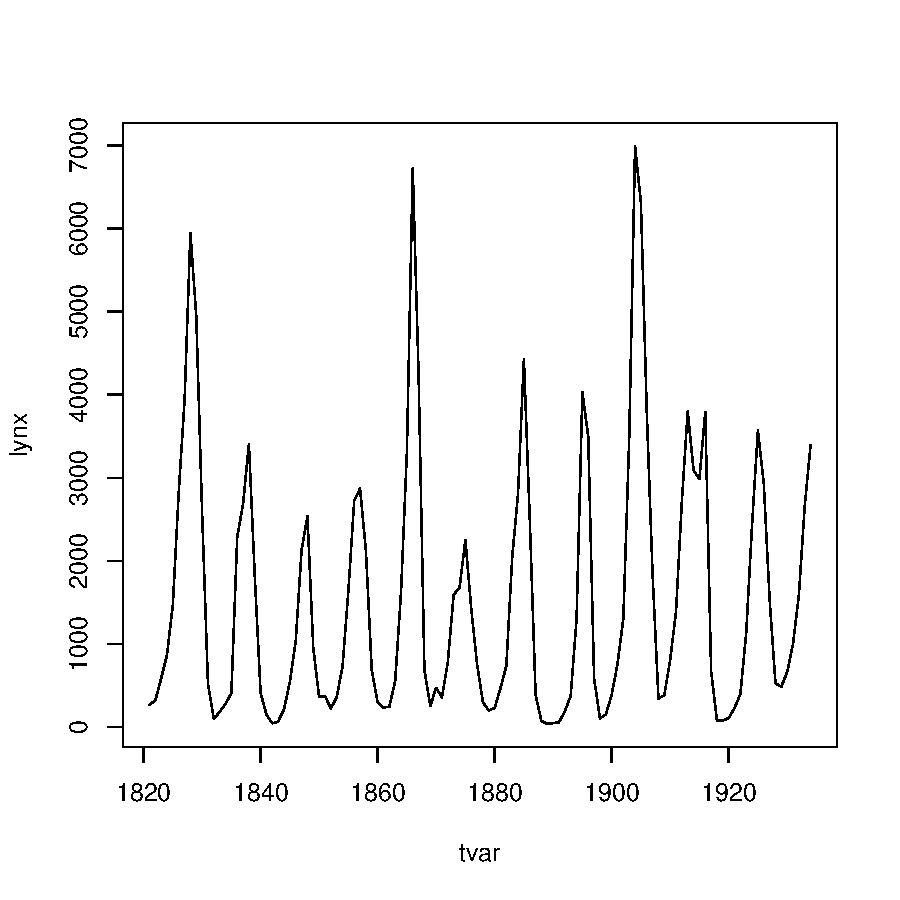
\includegraphics{figures/doby-033}

Suppose we want to estimate the cycle lengths. One way of doing this
is as follows:
\begin{Schunk}
\begin{Sinput}
R> yyy <- lynx>mean(lynx)
R> head(yyy)
\end{Sinput}
\begin{Soutput}
[1] FALSE FALSE FALSE FALSE FALSE  TRUE
\end{Soutput}
\begin{Sinput}
R> (sss <- subSeq(yyy,item=TRUE))
\end{Sinput}
\begin{Soutput}
   first last slength midpoint value
1      6   10       5        8  TRUE
2     16   19       4       18  TRUE
3     27   28       2       28  TRUE
4     35   38       4       37  TRUE
5     44   47       4       46  TRUE
6     53   55       3       54  TRUE
7     63   66       4       65  TRUE
8     75   76       2       76  TRUE
9     83   87       5       85  TRUE
10    92   96       5       94  TRUE
11   104  106       3      105  TRUE
12   112  114       3      113  TRUE
\end{Soutput}
\end{Schunk}

\begin{Schunk}
\begin{Sinput}
R> plot(tvar,lynx,type='l')
R> rug(tvar[sss$midpoint],col='blue',lwd=4)
\end{Sinput}
\end{Schunk}
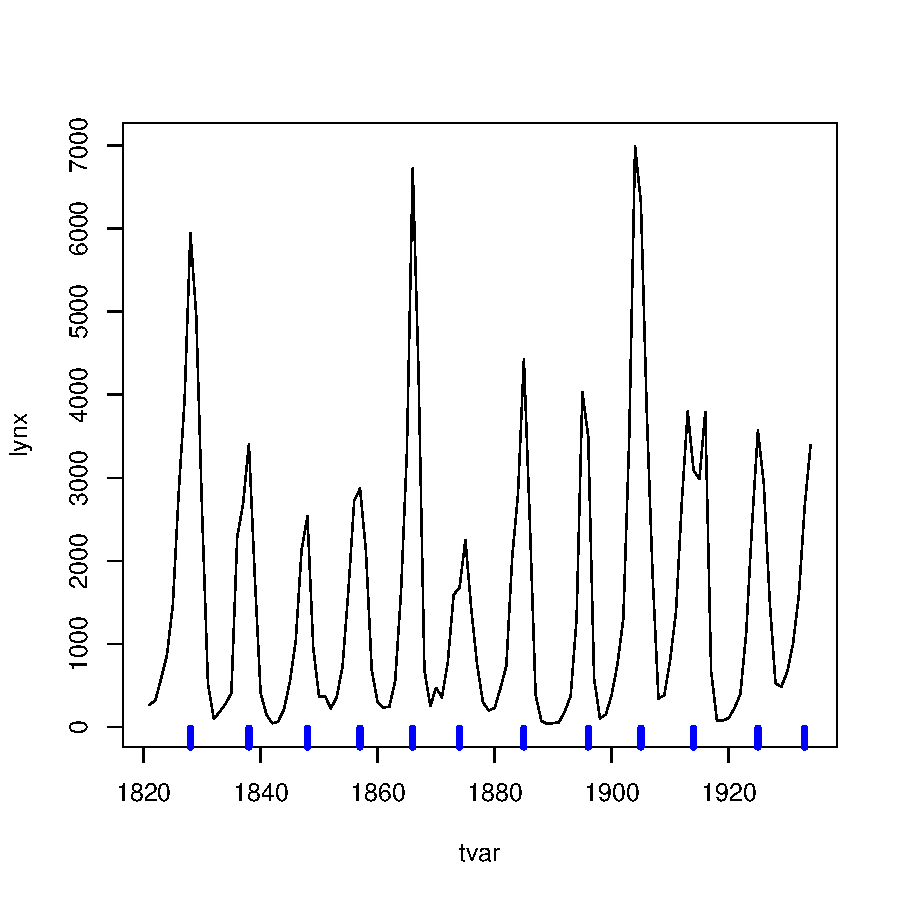
\includegraphics{figures/doby-035}

Create the 'event vector'
\begin{Schunk}
\begin{Sinput}
R> yvar <- rep(0,length(lynx))
R> yvar[sss$midpoint] <- 1
R> tse <- timeSinceEvent(yvar,tvar)
R> head(tse,20)
\end{Sinput}
\begin{Soutput}
   yvar tvar abs.tse sign.tse ewin run tae tbe
1     0 1821       7       -7    1  NA  NA  -7
2     0 1822       6       -6    1  NA  NA  -6
3     0 1823       5       -5    1  NA  NA  -5
4     0 1824       4       -4    1  NA  NA  -4
5     0 1825       3       -3    1  NA  NA  -3
6     0 1826       2       -2    1  NA  NA  -2
7     0 1827       1       -1    1  NA  NA  -1
8     1 1828       0        0    1   1   0   0
9     0 1829       1        1    1   1   1  -9
10    0 1830       2        2    1   1   2  -8
11    0 1831       3        3    1   1   3  -7
12    0 1832       4        4    1   1   4  -6
13    0 1833       5        5    1   1   5  -5
14    0 1834       4       -4    2   1   6  -4
15    0 1835       3       -3    2   1   7  -3
16    0 1836       2       -2    2   1   8  -2
17    0 1837       1       -1    2   1   9  -1
18    1 1838       0        0    2   2   0   0
19    0 1839       1        1    2   2   1  -9
20    0 1840       2        2    2   2   2  -8
\end{Soutput}
\end{Schunk}

We get two different (not that different) estimates of period
lengths:
\begin{Schunk}
\begin{Sinput}
R> len1 <- tapply(tse$ewin, tse$ewin, length)
\end{Sinput}
\begin{Soutput}
 1  2  3  4  5  6  7  8  9 10 11 12 
13 10  9  9  9  9 11 10  9 10 10  5 
\end{Soutput}
\begin{Sinput}
R> len2 <- tapply(tse$run,  tse$run, length)
\end{Sinput}
\begin{Soutput}
 1  2  3  4  5  6  7  8  9 10 11 12 
10 10  9  9  8 11 11  9  9 11  8  2 
\end{Soutput}
\begin{Sinput}
R> c(median(len1),median(len2),mean(len1),mean(len2))
\end{Sinput}
\begin{Soutput}
[1] 9.500 9.000 9.500 8.917
\end{Soutput}
\end{Schunk}

We can overlay the cycles as:
\begin{Schunk}
\begin{Sinput}
R> tse$lynx <- lynx
R> tse2 <- na.omit(tse)
R> plot(lynx~tae, data=tse2)
\end{Sinput}
\end{Schunk}
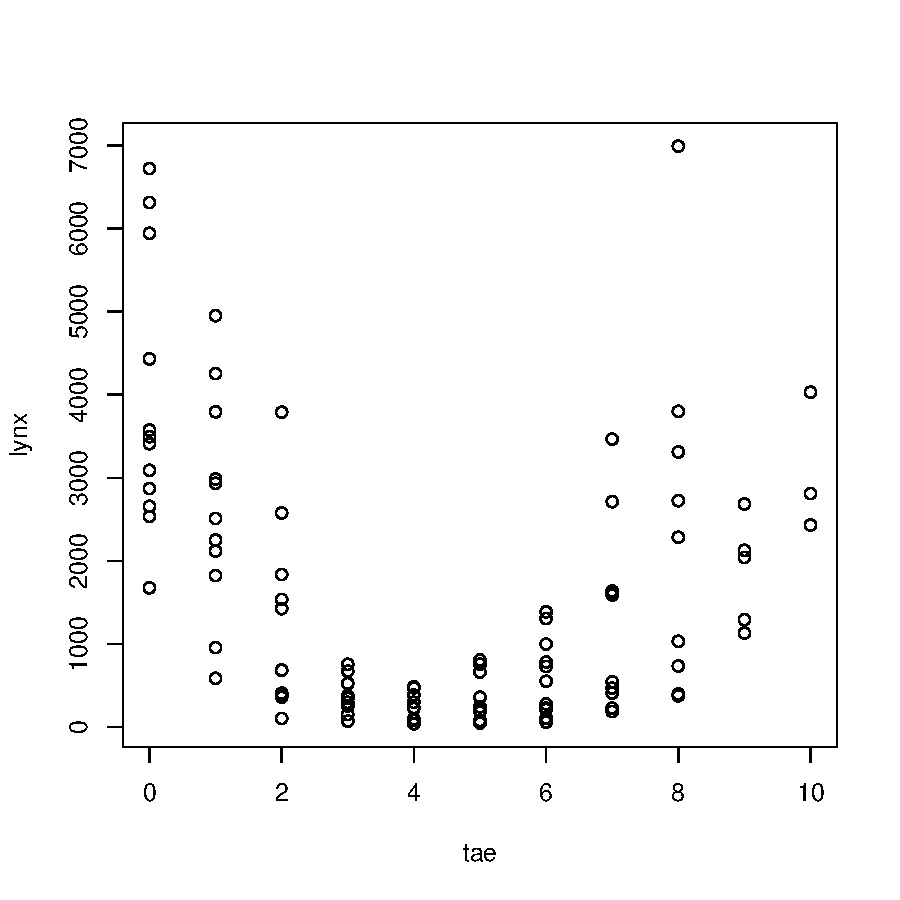
\includegraphics{figures/doby-038}

\begin{Schunk}
\begin{Sinput}
R> plot(tvar,lynx,type='l',lty=2)
R> mm <- lm(lynx~tae+I(tae^2)+I(tae^3), data=tse2)
R> lines(fitted(mm)~tvar, data=tse2, col='red')
\end{Sinput}
\end{Schunk}
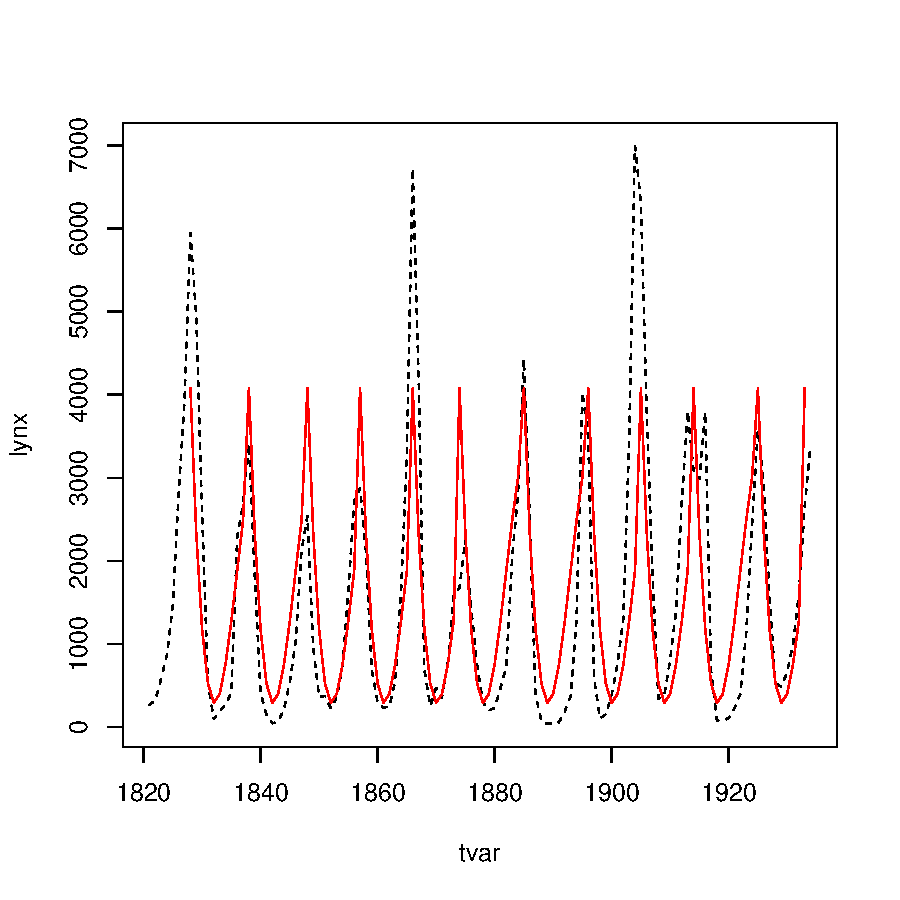
\includegraphics{figures/doby-039}



\def\esticon{\code{esticon()}}

\subsection[]{The \esticon\ function}
\label{esticon}

Consider a linear model which explains \code{Ozone} as a linear
function of \code{Month} and \code{Wind}:
\begin{Schunk}
\begin{Sinput}
R> data(airquality)
R> airquality <- subset(airquality, Month %in% c(5,6,7))
R> airquality <- transform(airquality, Month=factor(Month))
R> m<-lm(Ozone ~ Month * Wind, data=airquality)
R> coefficients(m)
\end{Sinput}
\begin{Soutput}
(Intercept)      Month6      Month7        Wind Month6:Wind 
     50.748     -41.793      68.296      -2.368       4.051 
Month7:Wind 
     -4.663 
\end{Soutput}
\end{Schunk}

When a parameter vector $\beta$ of (systematic) effects have been
estimated, interest is often in a particular estimable function, i.e.\
linear combination $\lambda^\top \beta$ and/or testing the hypothesis
$H_0: \lambda^\top \beta=\beta_0$ where $\lambda$ is a specific vector
defined by the user.

Suppose for example we want to calculate the expected difference in
ozone between consequtive months at wind speed 10 mph (which is about
the average wind speed over the whole period).

The \code{esticon} function provides a way of doing so.
We can specify several $\lambda$ vectors at the same time. For example

% @
% <<echo=T>>=
% Lambda <- rbind(
%   c(0,-1,0,0,0,0,-10,0,0,0),
%   c(0,1,-1,0,0,0,10,-10,0,0),
%   c(0,0,1,-1,0,0,0,10,-10,0),
%   c(0,0,0,1,-1,0,0,0,10,-10)
%   )
% @ %def


% @
% <<echo=T>>=
% Lambda <- rbind(
%   c(0,-1,0,0,0,0,-10,0,0,0),
%   c(0,1,-1,0,0,0,10,-10,0,0),
%   c(0,0,1,-1,0,0,0,10,-10,0),
%   c(0,0,0,1,-1,0,0,0,10,-10)
%   )
% @ %def

% @
% <<>>=
% esticon(m, Lambda)
% @ %def


% In other cases, interest is in testing a hypothesis of a contrast
% $H_0: \Lambda \beta=\beta_0$ where $\Lambda$ is a matrix. For example
% a test of no interaction between \code{Month} and \code{Wind} can be
% made by testing jointly that the last four parameters in \code{m} are
% zero (observe that the test is a Wald test):
% @
% <<echo=T>>=
% Lambda <- rbind(
%   c(0,0,0,0,0,0,1,0,0,0),
%   c(0,0,0,0,0,0,0,1,0,0),
%   c(0,0,0,0,0,0,0,0,1,0),
%   c(0,0,0,0,0,0,0,0,0,1)
%   )
% @ %def

% @
% <<>>=
% esticon(m, Lambda, joint.test=T)
% @ %def

For a linear normal model, one would typically prefer to do a
likelihood ratio test instead. However, for generalized estimating
equations of glm--type (as dealt with in the packages \pkg{geepack}
and \pkg{gee}) there is no likelihood. In this case \code{esticon}
function provides an operational alternative.

Observe that another function for calculating contrasts as above is the
\code{contrast} function in the \pkg{Design} package but it applies to
a narrower range of models than \code{esticon} does.


% \subsection{LSMEANS}
% \label{sec:xxx}


% Marginal means (also called population means or LSMEANS) can be
% calulated with \verb'lsmeans()'. See the documentation of  \verb'lsmeans()' for
% examples.


\section{Acknowledgements}
\label{discussion}

Credit is due to
Dennis Chabot, Gabor Grothendieck, Paul Murrell, Jim Robison-Cox  and Erik J{\o}rgensen for
reporting various bugs and making various suggestions to the
functionality in the \doby{} package.





%\VignettePackage{doBy}
%\VignetteIndexEntry{population means}
%\VignetteIndexEntry{LSMEANS}


%\RequirePackage{color,fancyvrb,amsmath,amsfonts}
%\DeclareMathOperator{\EE}{\mathbb{E}}

% \usepackage{framed}
% \usepackage{comment}
\definecolor{shadecolor}{gray}{0.91}
\def\R{\texttt{R}}
\def\code#1{\texttt{#1}}
\def\popmeans{\code{popMeans()}}
\def\popmatrix{\code{popMatrix()}}
\def\linmeans{\code{linMeans()}}
\def\linmatrix{\code{linMatrix()}}
\def\esticon{\code{esticon()}}

\section{A simulated dataset}
\label{sec:simulated-dataset}

Consider these data:
\begin{Schunk}
\begin{Sinput}
R> library(doBy)
R> dd <- expand.grid(A=factor(1:3),B=factor(1:3),C=factor(1:2))
R> dd$y <- rnorm(nrow(dd))
R> dd$x <- rnorm(nrow(dd))^2
R> dd$z <- rnorm(nrow(dd))
R> head(dd,10)
\end{Sinput}
\begin{Soutput}
   A B C        y        x        z
1  1 1 1 -0.61706 0.413575 -1.07969
2  2 1 1 -0.24555 0.500546 -1.16123
3  3 1 1 -1.82130 0.887302 -0.54921
4  1 2 1  0.11152 0.089367  1.08098
5  2 2 1  0.13153 0.853216 -0.03592
6  3 2 1 -1.09549 0.003458  0.86814
7  1 3 1 -0.83327 0.092064  3.49082
8  2 3 1 -0.17350 0.658494  0.24181
9  3 3 1  1.15572 1.364387 -1.33347
10 1 1 2  0.02867 1.746930 -0.05263
\end{Soutput}
\end{Schunk}

Consider the additive model
\begin{equation}
  \label{eq:1}
  y_i = \beta_0 + \beta^1_{A(i)}+\beta^2_{B(i)} + \beta^3_{C(i)} + e_i
\end{equation}
where $e_i \sim N(0,\sigma^2)$. We fit this model:

\begin{Schunk}
\begin{Sinput}
R> mm <- lm(y~A+B+C, data=dd)
R> coef(mm)
\end{Sinput}
\begin{Soutput}
(Intercept)          A2          A3          B2          B3 
    -1.4421      0.9119      0.7429      0.5020      1.0404 
         C2 
     1.1759 
\end{Soutput}
\end{Schunk}

Notice that the parameters corresponding to the factor levels
\code{A1}, \code{B1} and \code{C2} are set to zero to ensure
identifiability of the remaining parameters.


\section{Linear functions of parameters, contrasts}
\label{sec:line-funct-param}

For a regression model with parameters $\beta=(\beta^1, \beta^2,\dots,
\beta^P)$ we shall refer to a weighted sum of the form
\begin{displaymath}
  \sum_j w_j \beta^j
\end{displaymath}
as a contrast. Notice that it is common in the litterature to require
that $sum_j w_j=0$ for the sum $  \sum_j w_j \beta^j$ to be called a
contrast but we do not follow this tradition here.

The effect of changing the factor $A$ from \code{A2} to \code{A3} can
be found as
\begin{Schunk}
\begin{Sinput}
R> w <- c(0,-1,1,0,0,0)
R> sum(coef(mm)*w)
\end{Sinput}
\begin{Soutput}
[1] -0.1691
\end{Soutput}
\end{Schunk}

The \esticon\ function provides this estimate, the standard error
etc.\ as follows:
\begin{Schunk}
\begin{Sinput}
R> esticon(mm, w)
\end{Sinput}
\begin{Soutput}
  beta0 Estimate Std.Error t.value DF Pr(>|t|)  Lower  Upper
1     0  -0.1691    0.4978 -0.3396 12     0.74 -1.254 0.9155
\end{Soutput}
\end{Schunk}


\section{Population means}
\label{sec:xxx}

Population means (sometimes also called marginal means)
are in some sciences much used for reporting marginal effects (to be
described below). Population means are known as lsmeans in SAS
jargon. Population means is a special kind of contrasts as defined in
Section~\ref{sec:line-funct-param}.

The model (\ref{eq:1})
is a model for the conditional mean $\EE(y|A,B,C)$.  Sometimes one is
interested in quantities like $\EE(y|A)$. This quantity can not
formally be found unless $B$ and $C$ are random variables such that we
may find $\EE(y|A)$ by integration.

However, suppose that $A$ is a treatment of main interest, $B$ is a
blocking factor and $C$ represents days on which the experiment was
carried out. Then it is tempting to average $\EE(y|A,B,C)$ over $B$
and $C$ (average over block and day) and think of this average as
$\EE(y|A)$.

\subsection{A brute--force calculation}
\label{sec:xxx}

The population mean for $A=1$ is
\begin{equation}
  \label{eq:2}
  \beta^0 + \beta^1_{A1} + \frac{1}{3} (\beta^2_{B1}+\beta^2_{B2}+\beta^2_{B3})
  + \frac{1}{2}(\beta^3_{C1}+\beta^3_{C2})
\end{equation}

Recall that the
parameters corresponding to the factor levels
\code{A1}, \code{B1} and \code{C2} are set to zero to ensure
identifiability of the remaining parameters. Therefore we may also
write the population mean for $A=1$ as
\begin{equation}
  \label{eq:3}
  \beta^0 + \frac{1}{3} (\beta^2_{B2}+\beta^2_{B3})
  + \frac{1}{2}(\beta^3_{C2})
\end{equation}


This quantity can be estimated as:

\begin{Schunk}
\begin{Sinput}
R> w <- c(1, 0, 0, 1/3, 1/3, 1/2)
R> coef(mm)*w
\end{Sinput}
\begin{Soutput}
(Intercept)          A2          A3          B2          B3 
    -1.4421      0.0000      0.0000      0.1673      0.3468 
         C2 
     0.5880 
\end{Soutput}
\begin{Sinput}
R> sum(coef(mm)*w)
\end{Sinput}
\begin{Soutput}
[1] -0.34
\end{Soutput}
\end{Schunk}


We may find the population mean for all three levels of $A$ as
\begin{Schunk}
\begin{Sinput}
R> W <- matrix(c(1, 0, 0, 1/3, 1/3, 1/2,
+                1, 1, 0, 1/3, 1/3, 1/2,
+                1, 0, 1, 1/3, 1/3, 1/2),nr=3, byrow=TRUE)
R> W
\end{Sinput}
\begin{Soutput}
     [,1] [,2] [,3]   [,4]   [,5] [,6]
[1,]    1    0    0 0.3333 0.3333  0.5
[2,]    1    1    0 0.3333 0.3333  0.5
[3,]    1    0    1 0.3333 0.3333  0.5
\end{Soutput}
\begin{Sinput}
R> W %*% coef(mm)
\end{Sinput}
\begin{Soutput}
        [,1]
[1,] -0.3400
[2,]  0.5719
[3,]  0.4028
\end{Soutput}
\end{Schunk}

Notice that the matrix W is based on that the first level of $A$ is
set as the reference level. If the reference level is changed then so
must $W$ be.

\subsection[]{Using \esticon}
\label{sec:xxx}

Given that one has specified $W$, the \esticon\ function in the
\code{doBy} package be used for the calculations above and the
function also provides standard errors, confidence
limits etc:
\begin{Schunk}
\begin{Sinput}
R> esticon(mm, W)
\end{Sinput}
\begin{Soutput}
  beta0 Estimate Std.Error t.value DF Pr(>|t|)  Lower  Upper
1     0  -0.3400     0.352  -0.966 12   0.3531 -1.107 0.4269
2     0   0.5719     0.352   1.625 12   0.1302 -0.195 1.3388
3     0   0.4028     0.352   1.145 12   0.2747 -0.364 1.1697
\end{Soutput}
\end{Schunk}

\section[]{Using \popmatrix\  and \popmeans}
\label{sec:xxx}

Writing the matrix $W$ is somewhat tedious and hence error prone. In
addition, there is a potential risk of getting the wrong answer if the
the reference level of a factor has been changed.
The \popmatrix\ function provides an automated way of generating
such matrices.
The above \verb+W+ matrix is  constructed by
\begin{Schunk}
\begin{Sinput}
R> pma <- popMatrix(mm,effect='A')
R> summary(pma)
\end{Sinput}
\begin{Soutput}
     (Intercept) A2 A3     B2     B3  C2
[1,]           1  0  0 0.3333 0.3333 0.5
[2,]           1  1  0 0.3333 0.3333 0.5
[3,]           1  0  1 0.3333 0.3333 0.5
grid:
'data.frame':	3 obs. of  1 variable:
 $ A: chr  "1" "2" "3"
at:
 NULL
\end{Soutput}
\end{Schunk}



The \popmeans\ function is simply a wrapper around first a call
to \popmatrix\ followed by a call to (by default) \esticon:
\begin{Schunk}
\begin{Sinput}
R> pme <- popMeans(mm, effect='A')
R> pme
\end{Sinput}
\begin{Soutput}
  beta0 Estimate Std.Error t.value DF Pr(>|t|)  Lower  Upper A
1     0  -0.3400     0.352  -0.966 12   0.3531 -1.107 0.4269 1
2     0   0.5719     0.352   1.625 12   0.1302 -0.195 1.3388 2
3     0   0.4028     0.352   1.145 12   0.2747 -0.364 1.1697 3
\end{Soutput}
\end{Schunk}

More details about how the matrix was constructed is provided by the
\code{summary()} function:
\begin{Schunk}
\begin{Sinput}
R> summary(pme)
\end{Sinput}
\begin{Soutput}
  beta0 Estimate Std.Error t.value DF Pr(>|t|)  Lower  Upper A
1     0  -0.3400     0.352  -0.966 12   0.3531 -1.107 0.4269 1
2     0   0.5719     0.352   1.625 12   0.1302 -0.195 1.3388 2
3     0   0.4028     0.352   1.145 12   0.2747 -0.364 1.1697 3
Call:
NULL
Contrast matrix:
Length  Class   Mode 
     0   NULL   NULL 
\end{Soutput}
\end{Schunk}


The \verb+effect+ argument requires  to calculate the population means
for each level of
$A$ aggregating across the levels of the other variables in the data.

Likewise we may do:
\begin{Schunk}
\begin{Sinput}
R> popMatrix(mm,effect=c('A','C'))
\end{Sinput}
\begin{Soutput}
     (Intercept) A2 A3     B2     B3 C2
[1,]           1  0  0 0.3333 0.3333  0
[2,]           1  1  0 0.3333 0.3333  0
[3,]           1  0  1 0.3333 0.3333  0
[4,]           1  0  0 0.3333 0.3333  1
[5,]           1  1  0 0.3333 0.3333  1
[6,]           1  0  1 0.3333 0.3333  1
\end{Soutput}
\end{Schunk}
This gives the matrix for calculating the estimate for each
combination of \code{A} and \code{C} when averaging over \code{B}.
Consequently
\begin{Schunk}
\begin{Sinput}
R> popMeans(mm)
\end{Sinput}
\begin{Soutput}
  beta0 Estimate Std.Error t.value DF Pr(>|t|)   Lower  Upper
1     0   0.2116    0.2032   1.041 12   0.3183 -0.2312 0.6543
\end{Soutput}
\end{Schunk}
gives the ``total average''.


\subsection[]{Using the \code{at} argument}

We may be interested in finding the population means
at all levels of  $A$
but only at $C=1$. This is obtained by using the \code{at} argument:
\begin{Schunk}
\begin{Sinput}
R> popMatrix(mm,effect='A', at=list(C='1'))
\end{Sinput}
\begin{Soutput}
     (Intercept) A2 A3     B2     B3 C2
[1,]           1  0  0 0.3333 0.3333  0
[2,]           1  1  0 0.3333 0.3333  0
[3,]           1  0  1 0.3333 0.3333  0
\end{Soutput}
\end{Schunk}
Notice here that average is only taken over $B$. Another way of
creating the population means
at  all levels of $(A,C)$ is therefore
\begin{Schunk}
\begin{Sinput}
R> popMatrix(mm,effect='A', at=list(C=c('1','2')))
\end{Sinput}
\begin{Soutput}
     (Intercept) A2 A3     B2     B3 C2
[1,]           1  0  0 0.3333 0.3333  0
[2,]           1  1  0 0.3333 0.3333  0
[3,]           1  0  1 0.3333 0.3333  0
[4,]           1  0  0 0.3333 0.3333  1
[5,]           1  1  0 0.3333 0.3333  1
[6,]           1  0  1 0.3333 0.3333  1
\end{Soutput}
\end{Schunk}


We may have several variables in the \code{at} argument:
\begin{Schunk}
\begin{Sinput}
R> popMatrix(mm,effect='A', at=list(C=c('1','2'), B='1'))
\end{Sinput}
\begin{Soutput}
     (Intercept) A2 A3 B2 B3 C2
[1,]           1  0  0  0  0  0
[2,]           1  1  0  0  0  0
[3,]           1  0  1  0  0  0
[4,]           1  0  0  0  0  1
[5,]           1  1  0  0  0  1
[6,]           1  0  1  0  0  1
\end{Soutput}
\end{Schunk}

\subsection[]{Ambiguous specification when using the \texttt{effect} and
  \texttt{at} arguments}

There is room for an ambiguous specification if a variable appears in
both the \code{effect} and the \code{at} argument, such as
\begin{Schunk}
\begin{Sinput}
R> popMatrix(mm,effect=c('A','C'), at=list(C='1'))
\end{Sinput}
\begin{Soutput}
     (Intercept) A2 A3     B2     B3 C2
[1,]           1  0  0 0.3333 0.3333  0
[2,]           1  1  0 0.3333 0.3333  0
[3,]           1  0  1 0.3333 0.3333  0
\end{Soutput}
\end{Schunk}

This ambiguity is due to the fact that the \verb+effect+ argument asks
for the populations means at all levels of the variables but the
\verb+at+ chooses only specific levels.

This ambiguity is resolved as follows: Any variable in the \code{at}
argument is removed from the \code{effect} argument such as the
statement above is equivalent to
\begin{Schunk}
\begin{Sinput}
R> popMatrix(mm,effect='A', at=list(C='1'))
\end{Sinput}
\end{Schunk}

\subsection{Using covariates}

Next consider the model where a covariate is included:
\begin{Schunk}
\begin{Sinput}
R> mm2 <- lm(y~A+B+C+C:x, data=dd)
R> coef(mm2)
\end{Sinput}
\begin{Soutput}
(Intercept)          A2          A3          B2          B3 
    -1.4475      0.4126      0.3106      0.6511      0.8274 
         C2        C1:x        C2:x 
     1.9525      0.6242     -0.5630 
\end{Soutput}
\end{Schunk}

In this case we get
\begin{Schunk}
\begin{Sinput}
R> popMatrix(mm2,effect='A', at=list(C='1'))
\end{Sinput}
\begin{Soutput}
     (Intercept) A2 A3     B2     B3 C2   C1:x C2:x
[1,]           1  0  0 0.3333 0.3333  0 0.6603    0
[2,]           1  1  0 0.3333 0.3333  0 0.6603    0
[3,]           1  0  1 0.3333 0.3333  0 0.6603    0
\end{Soutput}
\end{Schunk}

Above, $x$ has been replaced by its average and that is the general
rule for models including covariates. However we may use the \code{at}
argument to ask for calculation of the population mean at some
user-specified value of $x$, say 12:
\begin{Schunk}
\begin{Sinput}
R> popMatrix(mm2,effect='A', at=list(C='1',x=12))
\end{Sinput}
\begin{Soutput}
     (Intercept) A2 A3     B2     B3 C2 C1:x C2:x
[1,]           1  0  0 0.3333 0.3333  0   12    0
[2,]           1  1  0 0.3333 0.3333  0   12    0
[3,]           1  0  1 0.3333 0.3333  0   12    0
\end{Soutput}
\end{Schunk}


\subsection{Using transformed covariates}

Next consider the model where a  transformation of a covariate is included:
\begin{Schunk}
\begin{Sinput}
R> mm3 <- lm(y~A+B+C+C:log(x), data=dd)
R> coef(mm3)
\end{Sinput}
\begin{Soutput}
(Intercept)          A2          A3          B2          B3 
  -1.248531    0.792032    0.737053    0.664020    1.055321 
         C2   C1:log(x)   C2:log(x) 
   0.955725    0.152552   -0.008265 
\end{Soutput}
\end{Schunk}

In this case we can not use \popmatrix\ (and hence
\popmeans\ directly.  Instead we have first to
generate a new variable, say \verb+log.x+, with
\verb+log.x+$=\log(x)$, in the data and then proceed as

\begin{Schunk}
\begin{Sinput}
R> dd <- transform(dd, log.x = log(x))
R> mm3 <- lm(y~A+B+C+C:log.x, data=dd)
R> popMatrix(mm3,effect='A', at=list(C='1'))
\end{Sinput}
\begin{Soutput}
     (Intercept) A2 A3     B2     B3 C2 C1:log.x C2:log.x
[1,]           1  0  0 0.3333 0.3333  0   -1.267        0
[2,]           1  1  0 0.3333 0.3333  0   -1.267        0
[3,]           1  0  1 0.3333 0.3333  0   -1.267        0
\end{Soutput}
\end{Schunk}

\section[]{The \code{engine} argument of \popmeans}

The \popmatrix is a function to generate a linear tranformation matrix of the model
parameters with emphasis on  constructing such matrices for population
means.
\popmeans\ invokes by default the \esticon\ function on this
linear transformation matrix for calculating parameter estimates and
confidecne intervals.
A similar function to \esticon\ is the \verb+glht+ function of the \verb+multcomp+
 package.

 The \code{glht()} function
 can be chosen via the \verb+engine+ argument of \popmeans:
\begin{Schunk}
\begin{Sinput}
R>  library(multcomp)
R> g<-popMeans(mm,effect='A', at=list(C='1'),engine="glht")
R> g
\end{Sinput}
\begin{Soutput}
	 General Linear Hypotheses

Linear Hypotheses:
       Estimate
1 == 0  -0.9280
2 == 0  -0.0161
3 == 0  -0.1851
\end{Soutput}
\end{Schunk}

This allows to apply the methods available on the \verb+glht+ object like
\begin{Schunk}
\begin{Sinput}
R> summary(g,test=univariate())
\end{Sinput}
\begin{Soutput}
	 Simultaneous Tests for General Linear Hypotheses

Fit: lm(formula = y ~ A + B + C, data = dd)

Linear Hypotheses:
       Estimate Std. Error t value Pr(>|t|)  
1 == 0  -0.9280     0.4064   -2.28    0.041 *
2 == 0  -0.0161     0.4064   -0.04    0.969  
3 == 0  -0.1851     0.4064   -0.46    0.657  
---
Signif. codes:  0 '***' 0.001 '**' 0.01 '*' 0.05 '.' 0.1 ' ' 1 
(Univariate p values reported)
\end{Soutput}
\begin{Sinput}
R> confint(g,calpha=univariate_calpha())
\end{Sinput}
\begin{Soutput}
	 Simultaneous Confidence Intervals

Fit: lm(formula = y ~ A + B + C, data = dd)

Quantile = 2.179
95% confidence level
 

Linear Hypotheses:
       Estimate lwr     upr    
1 == 0 -0.9280  -1.8135 -0.0424
2 == 0 -0.0161  -0.9016  0.8695
3 == 0 -0.1851  -1.0706  0.7004
\end{Soutput}
\end{Schunk}
which yield the same results as the \esticon\ function.

By default the functions will adjust the tests  and confidence intervals for multiplicity
\begin{Schunk}
\begin{Sinput}
R> summary(g)
\end{Sinput}
\begin{Soutput}
	 Simultaneous Tests for General Linear Hypotheses

Fit: lm(formula = y ~ A + B + C, data = dd)

Linear Hypotheses:
       Estimate Std. Error t value Pr(>|t|)
1 == 0  -0.9280     0.4064   -2.28     0.11
2 == 0  -0.0161     0.4064   -0.04     1.00
3 == 0  -0.1851     0.4064   -0.46     0.95
(Adjusted p values reported -- single-step method)
\end{Soutput}
\begin{Sinput}
R> confint(g)
\end{Sinput}
\begin{Soutput}
	 Simultaneous Confidence Intervals

Fit: lm(formula = y ~ A + B + C, data = dd)

Quantile = 2.732
95% family-wise confidence level
 

Linear Hypotheses:
       Estimate lwr     upr    
1 == 0 -0.9280  -2.0383  0.1824
2 == 0 -0.0161  -1.1264  1.0943
3 == 0 -0.1851  -1.2954  0.9252
\end{Soutput}
\end{Schunk}























\section{Discussion}
\label{sec:discussion}

 
\section{Acknowledgements}

This work was supported by the Danish National Advanced Technology
Foundation through the ILSORM project.

\bibliography{doBy-JSS}

\appendix


\end{document}



